% Use only LaTeX2e, calling the article.cls class and 12-point type.

\documentclass[12pt]{article}

% Users of the {thebibliography} environment or BibTeX should use the
% scicite.sty package, downloadable from *Science* at
% www.sciencemag.org/about/authors/prep/TeX_help/ .
% This package should properly format in-text
% reference calls and reference-list numbers.

\usepackage{scicite}

% Use times if you have the font installed; otherwise, comment out the
% following line.

\usepackage{times}

% The preamble here sets up a lot of new/revised commands and
% environments.  It's annoying, but please do *not* try to strip these
% out into a separate .sty file (which could lead to the loss of some
% information when we convert the file to other formats).  Instead, keep
% them in the preamble of your main LaTeX source file.


% The following parameters seem to provide a reasonable page setup.

\topmargin 0.0cm
\oddsidemargin 0.2cm
\textwidth 16cm 
\textheight 21cm
\footskip 1.0cm


%The next command sets up an environment for the abstract to your paper.

\newenvironment{sciabstract}{%
\begin{quote} \bf}
{\end{quote}}


% If your reference list includes text notes as well as references,
% include the following line; otherwise, comment it out.

\renewcommand\refname{References and Notes}

% The following lines set up an environment for the last note in the
% reference list, which commonly includes acknowledgments of funding,
% help, etc.  It's intended for users of BibTeX or the {thebibliography}
% environment.  Users who are hand-coding their references at the end
% using a list environment such as {enumerate} can simply add another
% item at the end, and it will be numbered automatically.

\newcounter{lastnote}
\newenvironment{scilastnote}{%
\setcounter{lastnote}{\value{enumiv}}%
\addtocounter{lastnote}{+1}%
\begin{list}%
{\arabic{lastnote}.}
{\setlength{\leftmargin}{.22in}}
{\setlength{\labelsep}{.5em}}}
{\end{list}}

\usepackage{amsthm}
\usepackage{thmtools}
\usepackage{enumerate}
\usepackage{amsfonts}
\usepackage{nth}
\usepackage{stackrel}
\usepackage{bbm}
\usepackage{amsmath}

\usepackage{graphicx}


\graphicspath{{./figures/}}

\theoremstyle{definition}
\newtheorem{mydef}{Definition.}[section]
\newtheorem{myexp}{Example.}[section]
\newtheorem{mycor}{\underline{Corollary}}[section]

\theoremstyle{plain}
\newtheorem{mythm}{Theorem}[section]
\newtheorem{mylemma}{Lemma}[section]
\newtheorem*{myproof}{Proof}
\newtheorem*{example}{example}


\setcounter{section}{-1}
\pagenumbering{arabic}

% Include your paper's title here

\title{ Introduction to Stochastic Process\\ STAT 615 Course Notes} 


% Place the author information here.  Please hand-code the contact
% information and notecalls; do *not* use \footnote commands.  Let the
% author contact information appear immediately below the author names
% as shown.  We would also prefer that you don't change the type-size
% settings shown here.

\author
{Daren Cline,$^{1\ast}$\\
\\
\normalsize{$^{1}$Department of Statistics, Texas A\&M University,}\\
\normalsize{College Station 77843-3143, USA}\\
\normalsize{ E-mail:  dcline@stat.tamu.edu.}
\\
\normalsize{Input by Tian Xia; Email: tianxia@cse.tamu.edu}
}

% Include the date command, but leave its argument blank.

\date{}



%%%%%%%%%%%%%%%%% END OF PREAMBLE %%%%%%%%%%%%%%%%



\begin{document} 

% Double-space the manuscript.

\baselineskip24pt

% Make the title.

\maketitle 



% Place your abstract within the special {sciabstract} environment.

\begin{sciabstract}
 
\end{sciabstract}




\section{Preliminaries}
\begin{mydef}
A \underline{\textbf{sample space}} $\mathbf{\Omega}$ is the collection of individual \underline{outcomes} or \underline{realizations} for a random experiment. \\
Subsets of $\mathbf{\Omega}$ are called \underline{events}. For $A \subset \mathbf{\Omega}$, we say ``A occurs'' if the outcome $\omega \in A$ 
\end{mydef}

$\Omega$ can be \underline{countable} (finite or countably infinite) or \underline{uncountable}. It need not consisit of real-valued entities. Most often, its role is in the background and simply assured.

\begin{myexp}
Toss a coin infinitely many times, observing $1$ (heads) or $0$ (tails) for each toss. The outcomes are inifinite sequences of $0$'s \& $1$'s, such as $(1,1,0,0,0,1, \cdots)$. The collection $\mathbf{\Omega}$ of all possible outcomes is uncountable in this case.
\end{myexp}
Events are subsets of $\mathbf{\Omega}$, often identified descriptively:
\begin{itemize}
\item ``\nth{1} toss is H''$=\{(x_1, x_2, \cdots):x_1 = 1\}$.
\item ``12 H's in the \nth{1} 100 tosses''  $=\{(x_1, x_2, \cdots): \sum_{i=1}^100 x_i = 12\}$.
\item ``the long tem proportion of H's is $\frac{1}{3}$''  =  $\{(x_1, x_2, \cdots):\frac{1}{n}\sum_{i=1}^n x_i \rightarrow \frac{1}{3}\}$.
\end{itemize}
A \underline{singleton} event is a subset of just one outcome, which is not quite the same as the outcome itself. \\
The empty set $\phi$ is considered to be an event also.

\begin{mydef}
A \underline{\textbf{probability measure}} $P$ is a set function (i.e. $P$ is applied to events, not to outcomes) such that
\begin{enumerate}[(i)]
\item $0 \leq P(A) \leq 1$, with $P(\mathbf{\Omega}) = 1, P(\phi) = 0$
\item if $A_1, A_2, \cdots$ are \underline{disjoint} then $P(\bigcup_{i=1}^\infty A_i) = \sum_{i=1}^\infty P(A_i)$ (similarly for finite unions) 
\end{enumerate}
\end{mydef}
when the $A_i$'s are not disjoint, we have
\begin{mythm}
(Boole's inequality) \[P(\bigcup_{i=1}^n A_i) \leq \sum_{i=1}^n P(A_i)\].
\end{mythm}

\begin{mydef}
A collection of $\mathbf{A}$ of subsets of $\mathbf{\Omega}$ is called a \underline{$\mathbf{\sigma}$\textbf{-algebra}} (or $\sigma$-field) if 
\begin{enumerate}[(i)]
\item $\phi, \mathbf{\Omega} \in \mathbf{A}$
\item $A \in \mathcal{A} \Longrightarrow   A^{\mathrm{c}} \in \mathcal{A}$
\item $A_1, A_2, \cdots \in \mathcal{A} \Longrightarrow \bigcup_{i=1}^\infty A_i \in \mathcal{A}$  (Some for finite unions) and hence also $\bigcap_{i=1}^\infty \in \mathcal{A}$ 
\end{enumerate}
\end{mydef}
\textbf{Note:} the requirement is closure under \underline{countable} unions and intersections. So a union of uncountably may subsets in $\mathcal{A}$ need not itself be in $\mathcal{A}$. (there are important mathematical reasons for allowing this.)
\textbf{Additional Note:} \underline{complement} $A^\mathcal{c}=$''A does not occur''
union of events $\bigcup_i A_i = $ ``some $A_i$ (at least one) occurs''
intersection $\bigcap_i A_i=$ ``every $A_i$ occurs'' 

\begin{myexp}
If $\mathbf{\Omega}$ is countable (such as the integers $\mathbb{Z}$) then we can let $\mathcal{A}$ be all subsets.
\end{myexp}
\begin{myexp}
If $\Omega = \mathbb{R}$ (all real values), we usually use the \underline{\textbf{Borel Sets}} $B=$ smallest $\sigma$-algebra that contains all singletons and all intervals. So $\mathcal{B}$ would include countable unions of intervals, but this by no means comes close to all it has. There is no direct formula or description to characterize all arbitrary Borel sets.\\
On the other hand, given $B \in \mathcal{B}$ and a probability measure $P$, $P(B)$ can be approximated as close as we like with the probability of some finite union of intervals.
\\ 
Borel sets on $\mathbb{R}^\mathrm{d}$ (d-dimensional vectors) are defined similaryly, using \underline{rectangles}.
\end{myexp}

\begin{myexp}
(cond.) Let $\Omega = \{(x_1, x_2, x_3, \cdots): x_i = 0$ or $x_i = 1$ for each $i \geq 1\}$ be the sample space of infinite sequences of coin tosses by \underline{cylinder events} (events where a \underline{finite} number of the $x_i$'s are fixed). For example, \[\{(x_1, x_2, \cdots) : x_1 = 1, x_2 = 0\}\].
\end{myexp}
The triple $(\Omega, \mathcal{A}, P)$ (i.e. sample space, $\sigma$-algebra of events probability measure) is called a \underline{probability space}. 

\begin{mydef}
A \underline{\textbf{random variable}} $X = X(\omega)$ is a real-valued function applied to outcomes (i.e., $X: \Omega \rightarrow \mathbb{R}$. \\
An \underline{extended random variable} can possibly take infinite values (i.e., $X: \Omega \rightarrow \bar{\mathbb{R}} \stackrel{def}{=} \mathbb{R} \vee \{-\infty, \infty\}$ (``$\stackrel{def}{=}$'' means ``defined as'', the same as ``$=:$''))
\end{mydef}


Since random variables (rvs) are functions, it is \underline{highly recommended} that you take care to distinguish them from actual (possible) values. We will usually, but not always, use upper case for rvs and lower case for actual values. (Also, try to avoid using the same name, such as $X$ or $Y$, for everything, and centatinly make distinctions between rvs in the same problem/context.) 

A \underline{random vector} is a vector of rvs and a \underline{random (stochastic) process} is a sequence of rvs (e.g. $(x_1, x_2, \cdots)$) or a function that takes random values (e.g. $x(t), t \in \mathbb{R}$, where each $X(t)$ is a random variable).

\begin{mydef}
Every rv $X$ has a \underline{cululative distribution function} (cdf) \[F_X(x) = P(X \leq x)\] (sensible even for extended rvs)
\end{mydef}

A rv $X$ (or its cdf) is \underline{discrete} if there is a countable set of values $\{a_i\}$ such that $\sum_i P(x = a_i) = 1, \{P_i\}=\{P(x = a_i)\}$ is called the \underline{probability mass function} (pmf). 

A rv $X$ (or its cdf) is \underline{absolutely continuous} if \[P(a < X \leq b) = F(b) - F(a) = \int_a^b f(x)dx\] for some function $f(x)$, called the \underline{probability density function} (pdf) 

\underline{However}, we do not with to limit ourselves to just two types. There are, for example, rvs with neither a pmf or a pdf, and these are mixtures of types. Things become more general still for random vectors. 

Furthermore, a stochastic process cannot be characterized so simply at all (More on this in the \nth{1} chapter). 

We will write $X \sim F_X$ (or $X \sim \{P_i\}$ or $X \sim f(x)$ when the context is clear) to signify that $X$ has distribution given by $F_x$. \\
\\
You should be familiar with all the commonly used distributions.
\begin{itemize}
\item ex. $Y \sim Poisson(\lambda)$ with pmf \[P(y = k) = \frac{\lambda ^k e^{- \lambda}}{k!}, k = 0, 1, 2, \cdots\].
\item ex. $T \sim Gamma(\alpha, \beta)$ with pdf \[f(t) = \frac{\beta ^ \alpha t^{\alpha - 1}e^{-\beta t}}{\Gamma (\alpha)}, t \geq 0\].
\end{itemize}

\begin{mydef}
Random variables $X_1, \cdots, X_m$ are \underline{independent} if \[P(X_1 \in A_1, X_2 \in A_2, \cdots, X_m \in A_m) = \prod_{i=1}^m P(X_i \in A)\] for all \textbf{Borel sets} $A_1, \cdots, A_m$. \\
Equivalently, \[P(X_1 \leq x_1, \cdots, X_m \leq x_m) = \prod_{i=1}^m P(X_i \leq x_i)\] for all real values $x_1, \cdots, x_m$. \\
(The \nth{1} definition can be applied to random elements of any kind, with appropriate $A_i$'s.)
\end{mydef}

A collection $\{X_t\}$ of rvs (possibly uncountably many) is \underline{independent} if every finite sub-collection is. That is, if $X_{t_1}, \cdots, X_{t_m}$ are independent, for any $t_1, \cdots, t_m$. \\ 

A sequence $\{X_n\}$ is \underline{independent and identically distributed} (iid) if it is independent and all the rvs have the same distribution. We sometimes write $\{X_n\} \stackrel{iid}{\sim} F$ (or just $X_n \stackrel{iid}{\sim} F$) . \\ 

Stochastic processes are generally \underline{not independent} (they wouldn't be interesting if they were). But they often can be constructed or described in terms of independent rvs. \\ 

Random variables and their distributions can also be characterized in terms of expectations. As before, we do not wish to be limited to special types (and in fact it is notationally more convenient not to be).

\begin{mydef}
Here is how the expectation $E(g(x))$ is defined (if possible).\\
For simplicity, just let $Y = g(X)$ and we'll define $E(Y)$.
\begin{enumerate}
\item \underline{indicator rv} \\ 

if 
\begin{displaymath}
Y = \mathbbm{1}_A = \begin{cases}
0, & \text{if A does not occur} \\
1, & \text{if A does occur}
\end{cases}
\end{displaymath}
then \[E(\mathbbm{1}_A) = P(A)\]. indicator rvs have \underline{Bernoulli distribution} (which simply means discrete on $\{0,1\}$)

\item \underline{simple rv} \\
Y is a finite linear combination of indicator rvs \\
i.e. $Y = \sum_{i=1}^m c_i \mathbbm{1}_{A_i}$ (hence discrete w/ finitely many values) \\
 then \[E(Y) = \sum_{i=1}^m c_i P(A_i)\]. (this works even if the $A_i$'s are not disjoint or if the $c_i$'s are not distinct.)
 
 \item \underline{nonnegative rv} \\ 
  $Y \geq 0$. There always exist nonnegative simple rvs $Y_n(\omega) \mathbbm{\uparrow} Y(\omega)$ for every $\omega \in \Omega$. \\
 Then \[E(Y) = \lim \limits_{n \rightarrow \infty} E(Y_n) \quad  \text{(which myght equal $\infty$)}\] 
 ( This does not depend on the choice of sequenc $\{Y_n\}$, nor is it necessarily the best way to \underline{compute} $E(y)$. )

\item \underline{general rv $Y$} \\
Define the positive part of $Y$, $Y_+ = \max(Y,0)$\\
and the negative part, $Y_- = \max(-Y, 0)$. \\
(both are nonnegative) \\
so $Y = Y_+ - Y_-$ and $|Y| = Y_+ + Y_-$\\
Then if either (or both) of $E(Y_+) \& E(Y_-)$ are finite, define \[E(Y) = E(Y_+)-E(Y_-)\]. (Again, the value can be infite - we just don't allow the case $\infty$ $-\infty$)
\end{enumerate}
\end{mydef}

The purpose of the above is just so we can define ( and talk about) expectations without having to worry about the type of rv or how the expectation is to be computed. In fact, computing expectations will depend on context and often is not necessary in specific cases.

\begin{mydef}
(Lebesque-Stielties notation). \\
If $X \sim F$, it is conventional to express \[E(x) = \int_{-\infty}^{\infty} x F(dx)\], and $E(g(x)) = \int_{-\infty}^{\infty}g(x)F(dx)$, when they can be defined. \\
A similar usage applies to random vectors, using a \underline{joint cdf} (but not to stochastic processes) .
\end{mydef}
$\mbox{}$\\
Other terminology. 
\begin{itemize}
\item A random variable $X$ is \underline{finite} if $|X(\omega)| < \infty$ for \underline{all} $\omega \in \Omega$. 
\item A random variable $X$ is \underline{bounded} if there exists a constant $C$ such that $|X(\omega)| \leq C$ for all $\omega \in \Omega$. 
\item Do not confuse ``finite'' \& ``bounded''. 
\end{itemize}

The terms apply in similar fashion to any real valued function $g(x)$.  \\ \\
An event $A$ occurs \underline{almost surely} (a.s.) or \underline{with probability 1} (w.p.1) if P(A) = 1. \\ 
Note that ``almost sure'' is in the context of a specific probability measure or model, whereas the definition of $A$ (as some event) is not. 

ex. $Y$ is almost surely finite if $P(|Y| < \infty) = 1$. However, the event $\{Y = \infty\}$ need not be empty. Indeed, we will want to discuss rvs taht are almost surely finite for some models but not for others ( and to identify the distinguishing condition ) . 

ex. $X_n$ converges to $X$ almost surely ($X_n \rightarrow X$ a.s.), if $P(\lim \limits_{n \rightarrow \infty}X_n = X) = 1$, \\
This is stronger than convergence in probability:  $P(|X_n - X| > \epsilon) \rightarrow 0$ for all positive $\epsilon$.


\subsection*{The basic limit theorems}
\begin{mythm}
\underline{\textbf{Monotone Convergence}} (MCT) \\
For $0 \leq X_n \mathbbm{\uparrow} X : E(X_n) \rightarrow E(X)$ (even if infinite) \\
Likewise, if $0 \leq g_n(x) \mathbbm{\uparrow} g(x)$ for all $x$, then \[\int g_n(x) dx \rightarrow \int g(x) dx\], and \[\sum_{i=1}^\infty g_n(i) \rightarrow \sum_{i=1}^\infty g(i) \]
\end{mythm}
\begin{mythm}
\underline{\textbf{Dominated Convergence}} (DCT) \\
For $X_n \rightarrow X$ such that $|X_n| \leq Y$ and $E(y) < \infty$, $E(X_n) \rightarrow E(X)$.\\
(again, similar statements for integrals \& sums)
\end{mythm}
\begin{mythm}
\underline{\textbf{Fatou's Lemma}} $X_n \geq 0, X_n \rightarrow X$ \[ \liminf \limits_{n \rightarrow \infty} E(X_n) \geq E(X)\] ( \& similarly for sums and integrals)\\
( Note: \[\liminf \limits_{n \rightarrow a_n} = \lim \limits_{n \rightarrow \infty} (\underset{k \geq n}{\inf} a_k) \quad \& \quad \limsup \limits_{n \rightarrow \infty} a_n = \lim \limits_{n \rightarrow \infty} (\underset{k \geq n}{\sup} a_k)\]. )
\end{mythm}
\begin{mythm}
\underline{\textbf{Strong Law of Large Numbers}} (SLLN) For iid $X_n$, \[\frac{1}{n}\sum_{i=1}^n X_i \rightarrow E(X) \qquad \text{(if defined)}\] almost surely, and \[E(|\frac{1}{n}\sum_{i=1}{n}X_i - E(X)|) \rightarrow 0 \quad \text{(if $E(|x|) < \infty$})\].
\end{mythm}

\subsection*{Equalities \& inequalities}

\begin{mythm}
$\mbox{}$
\begin{itemize}
\item If $X \geq 0$ then $E(X) = \int_0^\infty P(X > x)dx$, even if infinite (\& valid even if $P(X=\infty)>0$). 
\item If $X \geq 0$ and is integer-valued then \[E(X) = \sum_{n=0}^{\infty}P(X > n)\]
\end{itemize}
\end{mythm}

\begin{mythm} 
$\mbox{}$
\begin{enumerate}[(i)]
\item (Markov) If $g(x) \geq 0$ \& nondecreasing then \[P(X \geq x) \leq \frac{E(g(X))}{g(x)}\]  e.g. \[P(|X| >x) \leq \frac{E(|x|)}{x} \quad \& \quad P(|X| > x) \leq \frac{E(x^2)}{x^2}\].
\item $|E(x)| \leq E(|x|)$
\item (Lyapunov) $E(|X|^r) \leq (E(x^2)E(y^2))^{\frac{1}{2}}, \quad \text{if $0 < r <s$}$.
\item (Cauchy-Schwaiz) $|E(xy)| \leq (E(x^2)(y^2))^{\frac{1}{2}}$
\item (Jenson) If $g(x)$ is convex then $E(g(x)) \geq g(E(x))$ with equality only if $g(x)=a + bx$ for some constants $a,b$. \\
Note: ``convex'' means $g(ax+(1-a)y) \leq ag(x) + (1-a)g(y),0 < a < 1$ \\
Equivalently, $g(b) - g(a) = \int_{a}^{b}g'(u)du$ all $a,b$ and $g'(u)$ is nondecreasing (the derivative need not exist at all values of $u$ for this to hold)
\end{enumerate}
\end{mythm}
\begin{mythm}
(Kolmogorov maximal inequality) \\
If $X_n$ are independent, each $E(X_n^2) < \infty \quad \& \quad S_n = X_1 + \cdots + X_n$ \\
then \[P(\underset{k \leq n}{\max}|S_k - E(S_k)| > x) \leq \frac{\mathrm{Var}(S_n)}{x^2}\]
\end{mythm}
The next result takes many guises, but you should set the idea from examples shown.

\begin{mythm}
(Fubini-tonelli) \\
Suppose either that $g(x,y) \geq 0$ for all $x,y$ or the quantities below are \underline{finite} when $g(x,y)$ is replaced with $|g(x,y)|$.
\begin{enumerate}[(i)]
\item \[\iint g(x,y)dxdy = \iint g(x,y)dydx\].
\item \[\int \sum_{n=0}^\infty g(n,y)dy = \sum_{n=0}^\infty \int g(n,y) dy\].
\item \[\int E(g(X,y))dy = E(\int g(x,y)dy)\].
\item \[\sum_{n=0}^\infty E(g(X,n)) = E(\sum_{n=0}^\infty g(X,n))\].
\item \[\sum_{n=0}^\infty \sum_{k=0}^\infty g(n,k) = \sum_{k=0}^\infty \sum_{n=0}^\infty g(n,k)\].
\item \[\iint g(x,y)F(dx)G(dy) = \iint g(x,y)G(dy)F(dx)\], where the latter are lebesgue-stieltjes integrals. (When $g(x,y) \geq 0$ all $x,y$ the double integrals/sums/etc above can equal $\infty$, on both sides.)
\end{enumerate}
\end{mythm}

We rely heavily on conditional probabilities and conditional expectation. Like expectation, however, we want to discuss \& use them without being restricted to joint discrete distributions or joint continuous distributions. We provide here, without elaboration, a suitably general definition.

\begin{mydef}
Let $Y$ be a r.v. such that $E(Y)$ exists, and $X$ be a random element (r.v., r. vector, stochastic process). The \underline{conditional expectation} of $Y$ given $X$, denoted $E(y|X)$ is\\
a function of the random variable $X$, say $h(x)$, (Note: this also means $E(Y|X)$ is itself a r.v.) such that \[E(g(x)Y) = E(g(x)E(Y|X)) \qquad \text{(*)}\] for all (measurable) bounded real-valued functions $g(x)$. (``measurable'' just means $\{x:g(x) \leq y\}$ is a Borel set, which is a technical restriction not usually of much concern to us.)
\end{mydef}
Conditional Probability $P(y\in A | X) = E(\mathbbm{1}_A(y)|X)$. 

The definition \underline{does not} tell us how to compute $E(y|X)$; it merely says that we can define it.\\
Note that $E(y|X)$ is \underline{a random variable} (but it must be a function of $X$) . Often we may have a way to define or compute $h(x)=E(y|X=x)$ suitably and then set $E(y|X) = h(X)$.

\subsection*{Properties of conditional expectation}
\begin{mythm}
Given $X$, and r.v.'s $Y, Y_1, Y_2, \cdots$ (w/ means)
\begin{enumerate}[(i)]
\item $Y_1 \leq Y_2 \implies E(Y_1|X) \leq E(Y_2|X)$.
\item $E(aY_1 + bY_2|X) = aE(Y_1|X) + bE(Y_2|X)$.
\item MCT, DCT \& Fatou's lemma all hold, cond. on $X$.
\item The formula (*) in \textbf{Theorem.0.6.} holds whenever whenever the expectations exist (not just for bounded $g(x)$).
\item (Pull-Out) $E(g(x)y/X) = g(X) E(y|x)$, if it exists.
\item (In)equalities for expectation (Jensen, etc.) all hold, cond. on $X$.
\item If $Y$ is independent of X then $E(Y|X) = E(Y)$.
\item $y=h(x)$ then $E(y|x) = y$
\item (Tower) $E(y|x)=E(E(y|x,z)|x) = E(E(y|x)|x,z)$.
\end{enumerate}
Basically, we can work with conditional expectations in an intuitive fashion based on familarity with definitions for the case $(x,y)$ is jointly discrete or jointly absolutely cont. \\
But now we can do so without those restrictions, including the case $X$ is a stochastic process (or a portion of one) consisting of infinitely many rv's.
\end{mythm}
Take care to use the tower property, (ix) above, correctly. It is \underline{not} usually true that \[E(E(y|x)|z) = E(E(y|z)|x)\] 

One other caution: $E(y|x)$ is not originly defined since $P(b{x}=0)=1$ implies $E(y|x) + b(x)$ also satisfies the definition. We don't usually have a problem w/ this if there are only countably many r.v.s.

\newpage

\section{Introduction}
\begin{itemize}
\item definitions
\item examples (simple random walk, simple branching proc.)
\item probability generating functions
\item some analytic results
\end{itemize}

\begin{mydef}
A \underline{\textbf{stochastic process}} is a collection of random variables, $\{X_t\}_{t \in \mathbbm{T}}$, defined on the same probability space. The \underline{state space} $\mathbbm{X}$ is a set of possible values for $X_t$ and the \underline{index set} $\mathbbm{T}$ is the set on which $X_t$ evolves.\\
(a single instance of values $\{X_t\}$ is called a \underline{sample path}.) \\
For us, $\mathbbm{X}$ will usually be the integers $\mathbbm{Z}$ or the real line $\mathbbm{R}$ (or some other subset of $\mathbbm{R}$ but it can be $\mathbbm{R}^m$ or something more exotic. \\
$\mathbbm{T}$ will usually be the nonnegative integers $\mathbbm{Z}_+$ or the nonnegative real numbers $\mathbbm{R}_+ = [0, \infty)$, but it also can be more general. 
\end{mydef}

\begin{myexp}
$X_t=\#$ of people infected on day $t$ of an epidemic \\
$X_{s,t}=$ temperature at point $s$ on the globe and time $t$ \\
$X(A)=\#$ of fireant colonies in a region $A$ (here $\mathbbm{T}$ is a collection of sets, including all open \& closed sets)
\end{myexp}
$\mbox{}$\\
Stochastic processes have many applications: \\
e.g. signal process, random networks, queues, climate, earthquakes, insect populations, stock market, economics, epidemics, and so on. \\ \\
\textbf{Note}: I generally use upper case for random variables and lower case for actual values.\\ \\
Just as we do for a random variable \& a  random vector, we want to discuss the \underline{distribution} of a stochastic process. But, with infinitely many rv's, we cannot simply express it as an ordinary function (such as a cdf). Instead we have 
\begin{mythm}
The \underline{distribution} of a real-valued stochastic process $\{X_t\}$ (that is, how we can calculate probabilities \& expectations for it) is uniquely determined by its \underline{finite-dimensional distributions} \[F_{t_1, \cdots, t_n}(x_1, \cdots, x_n) = P(X_{t_1} \leq x_1, \cdots, X_{t_n} \leq x_n)\]
\end{mythm}
$\mbox{}$\\
The idea is that any probability about the process \underline{as a whole} can be computed in terms of limits involving finite-dim dist's (or prob's of finitely many rv's). \\
A corollary of this theorem is that, in principle, it is always possible to construct a process from its distribution in terms of functions of independent r.v's.
\begin{itemize}
\item ex. \[P(\sup_{n \geq 0} X_n \leq x) = \lim_{n \rightarrow \infty}P(\bigcap_{k=1}^n\{X_k \leq x\}) = \lim_{n \rightarrow \infty}F_{1, \cdots, n}(x, \cdots, x)\].
\item \[P(\mbox{the limit until $X_t$ first exceeds $x$ is finite}) = \sum_{n=0}^\infty P(\max_{k < n} X_k \leq x < X_n)\] (Respectively: limit of sums w/ finitely many terms, probability for finitely many r.v's)
\end{itemize}
$\mbox{}$\\
(Note: the concept applies to all stochastic processes, whether real-valued or not)\\ \\
\underline{key point} The individual random variables in a stochastic process are \underline{not independent}. Thus the primary problem is to \underline{model} their dependence. This can be done in various ways.
\begin{itemize}
\item[-]  by construction fron independent random variables\\
e.g. $X_t = \sum_{j=0}^\infty \lambda_j \epsilon_{t-j}$, where the $\epsilon_t$'s are iid.
\item[-] by conditional probabilities\\
e.g. $P(X_t = j | X_{t-1} = i) = {i \choose j}p^j (1-p)^{i-j}, i \geq j \geq 0$ 
\item[-] by correlation structure (which may not be sufficient to characterize the process) \\
e.g. $cov(X_t, X_{t-1})=p^j$
\end{itemize}
$\mbox{}$\\
Each approach offers insight into the process, so it is useful to study all three. Constructive versions of the process are also useful for simulations. Covariances are useful for statistics.
\begin{myexp}
\underline{Simple Random Walk} (SRW)
Let $S_n$ be a location at time $n$, on the integers $\mathbbm{Z}$ and suppose each new location is either up one or down one, at random, form the last location. Specifically,\begin{displaymath}\begin{aligned}&S_0 = 0 \\ &S_{n+1} = \begin{cases}S_n - 1 \quad \mbox{w.p. $1-p$}\\S_n + 1 \quad \mbox{w.p. $p$}\end{cases} \mbox{, $0 < p <1$}\end{aligned} \end{displaymath}
\end{myexp}
\begin{figure}[h]
\centering
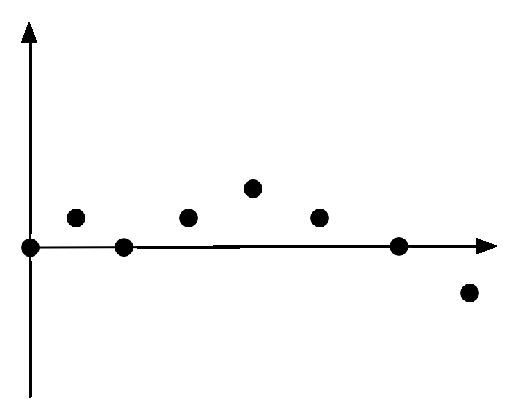
\includegraphics[scale=.5]{SRW.eps}
\caption{Simple Random Walk (SRW)}
\label{1:SRW}
\end{figure}
$\mbox{}$\\
Note that, no matter what the past history of the process is, the next step depends only on the current location. We can express this by
\begin{displaymath}
\begin{aligned}
P(S_{n+1} = j &| S_1 = i_1, \cdots, S_n = i_n) = \begin{cases} 1- p \quad \mbox{if $j = i_n - 1$}\\ p \quad \mbox{if $j = i_n + 1$}\\ 0 \quad \mbox{o.w.} \end{cases}\\  =& P(S_{n+1} = j | S_n = i_n) 
\end{aligned}
\end{displaymath}
A constructive definition is as follows: let $x_1, x_2, \cdots$ be iid r.v's with \[P(X_n = -1) = 1-p, \quad P(X_n = +1)=p\]. Then define $S_n = X_1 + \cdots + X_n$. $\{S_n\}$ is a simple random walk as defined above. (Here, $S_0 = 0$.)
\begin{myexp}
\underline{Simple Branching Process} (SBP) \\
Suppose at time $0$ one individual (the prognitor) is reproductive. At time $1$, this individual bears a random number $Z_{1,1}$ of descendants then becomes non-reproductive. Let $\{P_k\}_{k=0}^\infty$ be the probability mass function (pmf) for $Z_{1,1}$, i.e. \[P(Z_{1,1} = k) = p_k\]
\end{myexp}
At time 2, each newly born individual randomly bears offspring, independently of each other and with the same distribution as $Z_{1,1}$. Then each becomes non-reproductive. The process continues this way, with each new individual starting its own line of descent.
To represent the process constructively let $Z_{i,j}, \quad i \geq 1, j\geq 1$, ne iid r.v's with pmf $\{p_k\}$, and let \[Z_n = \mbox{total \# of individuals born at time $n$.}\] So
\begin{displaymath}
\begin{aligned}
Z_0 &= 1 \\
Z_1 &= Z_{1,1} \\
Z_2 &= Z_{2,1} + Z_{2,2} + \cdots + Z_{2, Z_1} \\
\vdots \\
Z_n &= Z_{n,1} + \cdots + Z_{n, Z_{n-1}}
\end{aligned}
\end{displaymath}
Each $Z_n$ is a \underline{random sum} of $Z_{n-1}$ id r.v's. (Define the sum to be $0$ if $Z_{n-1} = 0$.)
Note that each example relies on sums of independent r.v.' s. This is often the case for stochastic process (or approximately so) and at least makes a good starting point for our course. We review some basics about sums of independent r.v.'s.
\begin{mydef}
Let $\{a_n\}_{n=0}^\infty$ and $\{b_n\}_{n=0}^\infty$ be real valued sequences. Their \underline{convolution} is the sequence (double $\{a_n\} * \{b_n\}$) with elements \[\sum_{i=0}^n a_i b_{n-i}  = \sum_{i=0}^n a_{n-i}b_i\].
\end{mydef}
Note that $\{a_n\}*\{b_n\} = \{b_n\}*\{a_n\}$.

Also, $\quad (\{a_n\}*\{b_n\})*\{c_n\} = \{a_n\}*(\{b_n\}*\{c_n\})$ (check)
$\mbox{}$ \\
Convolutions have an important probabilistic interpretation, given next. Note: we write $X \sim \{a_n\}$ to indicate $X$ has pmf $\{a_n\}$. 
\begin{mylemma}
Suppose $X$ and $Y$ are independent r.v.'s such that $X$ has pmf $\{a_n\}$ and $Y$ has pmf $\{b_n\}$. Then $X+Y$ has pmf $\{a_n\}*\{b_n\}$. ($n \geq 0$)
\end{mylemma}
\begin{myproof}
(By asumption both $X$ \& $Y$ are nonnegative and integer valued.) \\
The event $\{X+Y=n\}$ can be decomposed into disjoint events: \[\{X+Y=n\}=\bigcap_{i=0}^n\{X=i, Y=n-i\}\] So \begin{displaymath} \begin{aligned}P(X+Y=n) &= \sum_{i=0}^n P(X=i)P(Y=n-i) \quad \mbox{using independence}\\ &= \sum_{i=0}^n a_i b_{n-i} \end{aligned} \end{displaymath}. That is, the pmf for $X+Y$ is $\{a_n\} * \{b_n\}$.
\end{myproof}
$\mbox{}$\\
\underline{\textbf{Remark}} If $X$ and $Y$ are independent and integer valued with pmf's $\{a_n\}_{n=-\infty}^\infty$, $\{b_n\}_{n=-\infty}^\infty$, rep. then \[P(X+Y=n) = \sum_{i=-\infty}^\infty a_i b_{n-i} \quad \mbox{(which exists since each sequence is summable)}\] (A probabilistic distribution is \underline{absolutely continuous} if it has a nonnegative density $f(x)$ such that $\int_{-\infty}^\infty f(x) dx = 1$. [There are continuous distributions w/o densities.]) Or if $X$ and $Y$ are independent with absolutely continuous distributions having densities $f_X(x)$ and $f_Y(y)$, rep., then $X+Y$ has density \[f_X * f_Y(Z) = \int_{-\infty}^\infty f_X(x)f_Y(z-x)dx\]. (Note: convolution formulas are context dependent, so beware!) \\
\underline{example} $\quad$ Suppose $X \sim Poisson(\lambda), Y \sim Poisson(\mu)$. So \[a_n = P(X=n) = \frac{\lambda^n e^{-\lambda}}{n!}, n \geq 0, b_n = P(Y = n) = \frac{\mu_n e^{-\lambda}}{n!}, n \geq 0\] Then, \[P(X+Y=n) = \sum_{i=0}^n a_i b_{n-i} = \cdots = \frac{(\lambda + \mu)^n e^{-(\mu + \lambda)}}{n!}, n \geq 0, \mbox{(check),} \quad \mbox{and $X+Y \sim Poisson(\lambda + \mu).$}\]
Note: If $X_1, \cdots, X_n$ are iid with pmf $\{p_k\}$ we will denote the pmf of $S_n = X_1 + \cdots + X_n$ by \[\{P_k^{*n}\} = \{p_k\}*\cdots * \{p_k\} \quad \mbox{(n-fold convolution)}\]. 
Computing convolutions can be tedious, difficult or even impossible. Alternatively, one may use a \underline{transform}. (there several different kinds of transforms.)

\begin{mydef}
\begin{enumerate}[(a)]
\item The \underline{generating function} (gf) for a sequence $\{a_n\}_{n \geq 0} a_n S^n$ is \[A(S) = \sum_{n=0}^\infty a_n S^n,\] (defined for all $S$ such that $\sum_{n=0}^\infty |a_n|S^n < \infty$.)
\item The probability generating function (pgf) for a pmf $\{p_n\}_{n \geq 0}$ is its gf: \[P(S) = \sum_{n=0}^\infty p_n S^n\]
\end{enumerate}
\end{mydef}
$\mbox{}$\\
\underline{\textbf{Remark}} $\quad$ If $X$ is a nonnegative  integer valued r.v. with pmf $\{P_n\}$. Then $P(s) = E(s^x), |s| \leq 1$. ($s \geq 0$ suffices here)\\
It often is more \underline{convenient} \& \underline{illuminating} to use this expectation notation.\\ 
examples \begin{itemize}
\item $X \sim Poisson(\lambda)$ \[E(s^x) = P(s) = \sum_{k=0}^\infty \frac{\lambda^k e^{-\lambda}s^k}{k!}=e^{\lambda s}e^{-\lambda} = e^{-\lambda(1-s)}\]
\item $X \sim binomial(n,p)$ \[E(s^x) = \sum_{k=0}^n {n \choose k} p^k (1-p)^{n-k} s^k = (ps + 1 - p)^n\]
\item $X \sim geometric(p)$ \[E(s^x) = \sum_{n=0}^\infty p(1-p)^k s^k = \frac{p}{1 - (1-p)s}\]
\end{itemize}
Some useful power series to know are
 \[\sum_{n=k}^\infty z^n = \frac{z^k}{1-z}\quad \mbox{if $|z| < 1$}\]
 \[\sum_{n=0}^m {m \choose n} b^{m-n}z^n = (z+b)^m\]
 \[\sum_{n=0}^\infty \frac{1}{n!} z^n = e^z\]
 \[\sum_{n=1}^\infty \frac{(-1)^{n-1}}{n}z^n = log(1+z) \quad \mbox{if $z > -1$}\]
An example solving a gf (rational polynomial, partial fractions)
\[A(s) = \frac{1 + s + 2s^2}{2-3s+s^2} = \frac{1 + s + 2s^2}{(2-s)(1-s)} = \frac{a + bs}{2-s} + \frac{c+ds}{1-s}\]
Solve the equation \[(a+bs)(1-s) + (c+ds)(2-s) = 1 + s + 2s^2\]
We have
\begin{displaymath}
\begin{aligned}
A(s) &=  \frac{-11}{2-s} + \frac{6-2s}{1-s}\\
       &=  \frac{-11/2}{1 - s/2} + \frac{6-2s}{1-s} \\
	&= \frac{-11}{2} \sum_{n=0}^{\infty} (s/2)^n + (6-2s)\sum_{n=0}^\infty s^n \\
	&= \sum_{n=0}^\infty [(-\frac{11}{2} 2^{-n} + 6)s^n - 2s^{n+1}] \qquad \mbox{(combining terms)} \\
	&= \frac{1}{2} + \sum_{n=1}^\infty (4 - 11(2^{-n-1})) \qquad  \qquad \mbox{($n=0$ case handled separately)} \\
\end{aligned}
\end{displaymath}
Hence, $a_0 = \frac{1}{2}$ \& $a_n = 4 - 11(2^{-n-1})$ for $n \geq 1$.

Note that all coefficients are nonnegative. Hence, all derivatives of $A(s)$ are nonnegative for $s\in [0,1)$. However, $A(1)=\infty$, meaning $\sum_{n=0}^\infty a_n = \infty$.\\ \\
recursion method \\
Fibonacci Sequence $f_0 = f_1 = 1$ and $f_n = f_{n-1} + f_{n-2}, n \geq 2$ let 
\begin{displaymath}
\begin{aligned}
F(s) &= \sum_{n=0}^{\infty} f_n s^n = 1 + s + \sum_{n=2}^\infty (f_{n-1} + f_{n-2})s^n \\
      &= 1 + s + s(F(s) - 1) + s^2F(s)\\
      & \implies F(s) = \frac{1}{1-s-s^2}
\end{aligned}
\end{displaymath}
using the method on the previous page,
\begin{displaymath}
\begin{aligned}
F(s) &= \frac{1}{s_2 - s_1} (\frac{1}{s - s_2} - \frac{1}{s - s_1}) = (\frac{s_1}{1 + s_1 s} - \frac{s_2}{1 + s_2 s})\frac{-1}{s_2 - s_1} \\
&= \frac{-1}{\sqrt{5}}(\sum_{n=0}^\infty s_1 (-s_1 s)^n - \sum_{n=0}^\infty s_2 (-s_2 s)^n) \quad \mbox{(geom. series)} \\
&= \sum_{n=0}^\infty \frac{1}{\sqrt{5}}((\frac{1+\sqrt{5}}{2})^{n+1} - (\frac{1-\sqrt{5}}{2})^{n+1})
\end{aligned}
\end{displaymath}
Therefore, $f_n = \frac{1}{\sqrt{5}}((\frac{1 + \sqrt{5}}{2})^{n+1} - (\frac{1-\sqrt{5}}{2})^{n+1})s^n$ for all $n \geq 0$. (doublecheck: $f_0 = 1, f_1=1,$ etc.\\ \\
\underline{\textbf{Remark}} $\quad$ Note the relationship between a pgf and the \underline{moment generating function} of $X$: \[m(t) = E(e^{tx}) = P(e^t)\]. (pgf's are relevant only for integer valued r.v's, but mgf's are more general) \\
\underline{\textbf{Another Remark}}: for a doubly infinite sequence $\{a_n\}_{n=-\infty}^\infty$. We can have the gf $A(s)=\sum_{n=-\infty}^\infty a_n s^n$, as long as existence $(\sum_{-\infty}^\infty |a_n| s^n < \infty)$ is not a problem. \\ \\
We now recall some of the basic properties of gf's
\begin{mythm}
Let $A(s) = \sum_{n=0}^\infty s^n, B(s) = \sum_{n=0}^\infty b_n s^n$, and assume existence
\begin{enumerate}[(i)]
\item Suppose $\sum_{n=0}^\infty |a_n| s_0^n < \infty$, then for all $s \in (-s_0, s_0)$ [The condition allows us to bring derivative inside the sum.] \[\frac{d}{ds}A(s) = \sum_{n=1}^\infty n a_n s^{n-1}\].
\item $A(s)$ is infinitely differentiable on $(-s_0, s_0)$.
\item $\{a_n\}$ is uniquely determined by its gf (This is a crucial point as it says there is a 1-1 correspondence between sequences \& their gf's (assuming existence of the gf). This is why $A(s)$ is called ``generating''): \[a_n = \frac{1}{n!} (\frac{d^n}{ds^n}A(s))_{s=0}\]
\item If every $a_n \geq 0$, then $A(s)$ is non decreasing for $s \geq 0$ and all derivatives of $A(s)$ are non decreasing for $s \geq 0$.\\
In particular, A(s) is \underline{convex}: \[\alpha A(x) + (1-\alpha) A(y) \geq A(\alpha x + (1-\alpha)y) \quad (0 \leq \alpha \leq 1)\]
\item The gf for $\{a_n\}*\{b_n\}$ is $A(s)B(s)$. In review of (iii), $A(s)B(s)$ thus can be used to identify the convolution.  $\quad \square$ 
\end{enumerate}
\end{mythm}
$\mbox{}$\\
Now we want to look at how these properties are relevant to integer valued r.v.'s.\\
But first an extension.
\begin{mydef}
An \underline{\textbf{extended}} r.v. is a random variable that can possibly take values $+\infty$ or $-\infty$. \\
In particular, suppose $X$ is nonnegative but extended. \\
Then its cdf $F(x)=P(X \leq x)$ satisfies $\lim_{x \rightarrow \infty} F(x) = P(X \leq x)$, which could be less than 1. The ``missing'' probability is $P(X = \infty)$.
\end{mydef}
$\mbox{}$\\
Why would we consider such rv's? Interestingly, they appear all too easily in stochastic process. \\ \\
\textbf{EX 1.2} (cont) SRW $S_n = X_1 + \cdots + X_n$ where $X_n \sim$ iid with $P(X_n = 1)=p = 1- P(X_n = -1)$. \\
Let $\mathcal{T}_k = \min \{n:S_n = k\}$, the time that value $k$ is first "hit" by the process.\\
The problem is that there are sequences for which $k$ is never hit: 
\begin{figure}[h]
\centering
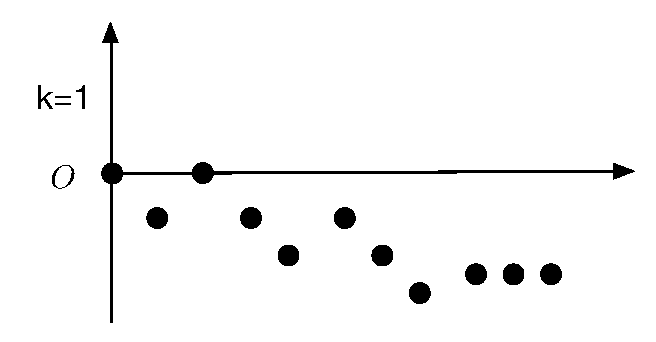
\includegraphics[scale=.5]{SRW2.eps}
\caption{Simple Random Walk (SRW) never hit}
\label{1:SRW2}
\end{figure}
For those cases, we naturally define $\mathcal{T}_k = \infty$. \\
\textbf{EX 1.3} (cont.) SBP $Z_n$. Recall $Z_0 = 1$. Since $Z_{n-1}=0\implies Z_n=0$, we call $\mathcal{T}_0 = \min\{n: Z_n =0\}$. The \underline{extinction time} of the process. Again, this may never happen in which case $\mathcal{T}_0 = \infty$. \\ \\
Batch to pdf's.

\underline{convention} for pgf's: defined for $0 \leq s < 1$. values at 1 are defined as limits as $s \uparrow 1$.
\begin{mythm}
Suppose $X$ is nonnegative integer valued and possibly extended, with pmf $P_n = P(X=n),n=0,1,2,\cdots$
\begin{enumerate}[(i)]
\item \[P(1) = \sum_{n=0}^\infty P_n = P(X < \infty)\]. Note: This is also $\lim_{s \uparrow 1}P(s)$. $P(X = \infty)$ is not in the sum. $s^\infty = 0$ when $0 \leq s < 1$. \\
\textbf{Remark}: $P(X < \infty)=1$ does not imply $X$ is always finite.
\item $P(s)$ is infinitely differentiable, nondecreasing and all its derivatives are nondecreasing. In particular, it is convex.
\item For all $n$, \[P_n = \frac{1}{n!}(\frac{d^n}{ds^n}P(s))_{s=0}\]. Thus $P_n$ is uniquely determined by its pgf.
\item (\underline{Factorial Moments}) \underline{\underline{Assume $P(1)=1$}}. \\
Then \[(\frac{d^n}{ds^n}P(s))_{s\uparrow 1} = E(X(X-1)\cdots(X-n+1)\]. $s \uparrow 1$ defined as limit since derivatives may not exist for $s \geq 1$ \\
\underline{prob. proof}: (To be rigorous, we should also justify why it is okay to bring the derivative inside the expectation for this case. However, note how the prob. proof (using expectation) gives more insight than the analytic proof would.)
\begin{displaymath}
\begin{aligned}
\frac{d^n}{ds^n} P(s) &= \frac{d^n}{ds^n} E(s^X) \\
		&= E(\frac{d^n}{ds^n}s^X) = E(X(X-1)\cdots(X-n+1)s^{X-n}) \\
		&\stackrel{s\uparrow 1}{\rightarrow} E(X(X-1)\cdots(X-n+1)\mathbbm{1}_{x < \infty}),\quad \mbox{($\mathbbm{1}_{X < \infty} =1$ if $X < \infty, -0$ o.w.)} \\
		&=E(X(X-1)\cdots(X-n+1)) \quad \mbox{(since $P(1)=1 \implies P(X < \infty)=1$)}\\
\end{aligned}
\end{displaymath}
\underline{analytic proof}: use Thm.1.2(i)
\item Suppose $Y$ is also nonnegative integer valued with pdf $Q(s)$. If $X$ and $Y$ are \underline{\underline{independent}} then $X+Y$ has pgf $P(s)Q(s)$.\\
\underline{prob. proof}: the pgf for $X+Y$ is
\begin{displaymath}
\begin{aligned}
E(s^{X+Y}) &= E(s^Xs^Y)\\
	&= E(s^X)E(s^Y) \quad \mbox{by independence} \\
	&= P(S)Q(S) 
\end{aligned}
\end{displaymath}. (note how we avoided referring to the convolution.) $\quad\square$
\end{enumerate}
\end{mythm}
$\mbox{}$\\
\begin{mycor}
 If $X$ has pgf $P(s)$ and \underline{\underline{$P(1)=1$}} then $E(x)=P'(1)$ and $Var(X) = P''(1)+P'(1)-(P'(1))^2$, (where the derivatives $P'(1)$ \& $P''(1)$ are computed as limits with $s \uparrow 1$ if necessary).
\end{mycor}
\begin{myproof}
(check - revisit Thm 1.3 (iv).)\\
(exercise -what is $P'(1)$ when $P(1) < 1$? It can still be finite.) $\quad \square$
\end{myproof}
\begin{example}
$X \sim Pois(\lambda). Y \sim Pois(\mu)$, independent (both are finite w.p.1)\\
We have seen 
\begin{displaymath}
\begin{aligned}
&E(s^X) = e^{-\lambda (1-s)}, E(s^Y) = e^{-\mu(1-s)} \\
\frac{d}{ds} &e^{-\lambda(1-s)} = \lambda e^{-lambda (1-s)} \rightarrow \lambda \quad \mbox{as} \quad s \rightarrow 1 \mbox{. So} \quad E(x) = \lambda \\
\frac{d^2}{ds^2}&e{-\lambda(1-s)} = \lambda^2 e^{-\lambda(1-s)} \rightarrow \lambda^2 \quad \mbox{as} \quad s \rightarrow 1 \mbox{. So} \quad E(X(X-1)) = \lambda^2 \\
\end{aligned}
\end{displaymath}
and $Var(X) = \lambda^2 + \lambda - \lambda^2 = \lambda$. \\
$X + Y$ has pgf 
\begin{displaymath}
\begin{aligned}
&e^{-\lambda(1-s)}e^{-\mu(1-s)} \quad \mbox{by Thm.1.3(v)} \\
= &e^{-(\lambda + \mu)(1-s)} \\
 \implies &X+Y \sim Pois(\lambda + \mu) \quad \mbox{by Thm.1.3 (iii)}
\end{aligned}
\end{displaymath}
\end{example}
\begin{example}
$X \sim bin(n,p), Y \sim bin(m,p)$, indep. \\
(use pgf's to show $E(X) = np$, $Var(X) = np(1-p)$ and $X+Y \sim bin(n+m, p)$.) 
\end{example}
$\mbox{}$\\
\underline{\textbf{EX.1.2} cont.}  SRW $S_n = X_1 + \cdots + X_n$.\\
The pgf for each $X_\mu$ is 
\begin{displaymath}
\begin{aligned}
P(s) = E(s^{X_k}) &= sP(X_k = 1) + s^{-1}P(X_k = -1) \\
			&= ps + (1-p)s^{-1}
\end{aligned}
\end{displaymath}
There is no problem with existence, so we still have 
\begin{displaymath}
\begin{aligned}
E(s^{S_n}) &= E(S^{X_1 + \cdots + X_n}) \\
&=E(s^{X_1}) \cdots E(s^{X_n}) \quad \mbox{by independence}\\
&= (P(s))^n = (ps + (1-p)s^{-1})^n
\end{aligned}
\end{displaymath}. Observe that this is \[\sum_{k = -n}^n P(S_n = k)s^k \quad \mbox{, which includes both pos. \& neg. k.}\] (Note: $\frac{S_n + n}{2} \sim bin(n,p)$ - check; there are several ways you can do this.)
\begin{mythm}
Suppose $X_1, X_2, \cdots$ is a sequence of r.v.'s and $N$ is a nonnegative integer valued r.v., independent of the sequence. The r.v. $S_N = X_1 + \cdots + X_n$ ($=0$ if $N=0$ by convention) is called a \underline{random sum} of the sequence. $\quad \square$
\end{mythm}
$\mbox{}$\\
We have already seen an example of random sums in our construction of the simple branching process. (Ex.1.3).
\begin{mythm}
Suppose $X_1, X_2, \cdots$ are iid with pgf $P(s) = \sum_{k=0}^\infty P_k s^k$ and $N$ has pgf $A(s)=\sum_{n=0}^\infty a_n s^n$, $N$ independent of $\{X_n\}$. Then $S_N = X_1 + \cdots + X_N$ has pgf $A(P(s))$, $  0 \leq s \leq 1$.
\end{mythm}
$\mbox{}$\\
prob. proof. (by and expectation) Assume $0 \leq s \leq 1$.\\
Recall that the pgf of $S_n$ of $S_n$ is $E(s^{S_n}) = (P(s))^n$. \\
This even makes sense if $n=0$ (since $S_0 = 0$ by convention).
Thus $E(s^{S_N}|N) = (P(s))^N$ (note: this is a function of $N$)\\ 
(\textbf{Important}: Regardless of the type of rv's, we can think of $E(X|Y)$ as the \underline{function of Y} such that \[E(h(Y)X) = E(h(Y)E(X|Y)\], whenever the expectations make sense. )\\ 
By the law of iterated expectation 
\begin{displaymath}
\begin{aligned}
E(s^{S_N}) &= E(E(s^{S_N}|N)) \\
		&=E((P(s))^N) = A(P(s)) \\
\end{aligned}
\end{displaymath}
(take limit as $s\uparrow 1$ to get case $s=1$.) \\
\textbf{Be sure to learn both these methods ($\uparrow \downarrow$)} \\
prob. proof (by partitioning the sample space)\\
Using the indicator functions,
\begin{displaymath}
\begin{aligned}
E(s^{S_N}) & = E(\sum_{n=0}^\infty s^{S_n} \mathbbm{1}_{N=n}) \\
		&= \sum_{n=0}^\infty E(s^{S_n})E(\mathbbm{1}_{N=n}) \quad \mbox{(by independence of $S_n \in N$)}\\
		&= \sum_{n=\infty}^\infty (P(s))^n a_n \qquad \mbox{(since $E(\mathbbm{1}_{N=n} = P(N=n) = a_n$)} \\
		&= A(P(s))  \qquad \qquad \qquad\qquad\qquad\qquad\qquad \qquad \qquad \square
\end{aligned}
\end{displaymath}

Refer to Resnick for an analytical proof involving the pmf of $S_N$, given by \[P(S_n = j) = \sum_{n=0}^\infty P_j^{*n} a_n\], where $P_j^{*n} = P(S_n = j)$ (n-fold convolution) and \\
$\mbox{}\qquad \quad P_j^{*0} = P(S_0 = j) = \begin{cases} 1 \quad \mbox{if $j=0$} \\ 0 \quad \mbox{o.w.}\end{cases}$
\begin{mycor}
Assume as in Thm.1.5. If $E(|X_1|) < \infty$ and $P(N < \infty) = 1$ then \[E(S_N) = E(N)E(X_1) \quad \mbox{(this is valid even if $E(N) = \infty$})\]. If also $E(X_1^2) < \infty$ and $E(N^2) < \infty$ then \[Var(S_N) = E(N)Var(X_1) + Var(N)(E(X_1))^2\].
(Helpful result: variance partition formula $var(X) = E(var(X|Y)) + var(E(X|Y))$.)
\end{mycor}
\begin{myproof}
(exercise - use the pgf from Thm1.11, or compute directly using either of the methods in the proof of Thm.1.5.) $\quad \square$
\end{myproof}
$\mbox{}$ \\
\underline{EX.1..3 (cont.)} Simple Branching Process \\
Let $Z_{ij}$ be iid with pmf $\{p_k\}$ and pgf $P(s)$. \\
Recall that $Z_0 = 1, Z_1 = Z_{1,1}, \cdots, Z_n = Z_{n,1} + \cdots + Z_{n, Z_{n-1}}, \cdots$ \\
Note that $Z_{n-1}$ depends only on $Z_{ij}$'s s.t. $i \leq n-1$ and thus $Z_{n-1}$ is independent of $Z_{n,j}$'s. \\
Therefore $Z_n$ is a random sum of $Z_{n,j}$'s (w/ $N = Z_{n-1}$) and so its pgf is $P_n(s) = E(s^{Z_n})$ where $P_1(s) = P(s)$ and \begin{displaymath}
\begin{aligned}
P_n(s) &= P_{n-1}(P(s)) \\
&= \cdots = P(P(\cdots P(s) \cdots)). \quad \mbox{(n-fold composition)} 
\end{aligned}
\end{displaymath}
(interpret $P_n(s) = P(P_{n-1}(s))$: think of $z_1$ independent process starting at time 1.) [Many problems can be solved by ``conditioning''. There may be several ways to do this. (In this situation, one cond. on $Z_{n-1}$, the other cond. on $Z_1$)] \\
\begin{example}
Let $P(s) = 1-p + ps$ (pgf of $Bernoulli(p)$) \\
Thus, at each generation the (sole) individual either generates one offspring, w.p. p, or none at all (which stops the process). \\
$\mbox{}$\\
Thinking prpbabilistically:  $\quad Z_n = 1  \quad \mbox{iff $n$ independent successes (births) have occurred (w.p $p^n$)}$ \\
				$\mbox{}\qquad\qquad\qquad\qquad\qquad\qquad$ $Z_n = 0$ o.w.  (w.p. $1-p^n$) \\
Thinking analytically: We claim $P_n(s) = 1 - p^n + p^ns$ \\
Proof by induction:    $P_1(s) = P(s) = 1 - p + ps$ \\
			     $\mbox{} \quad \qquad \qquad \qquad \qquad$	If we claim holds for $P_n$ then
\end{example}






























\bibliography{scibib}

\bibliographystyle{Science}

\clearpage



\end{document}




















